%%%%%%%%%%%%%%%%%%%%%%%%%%%%%%%%%%%%%%%%%
% University Assignment Title Page 
% LaTeX Template
% Version 1.0 (27/12/12)
%
% This template has been downloaded from:
% http://www.LaTeXTemplates.com
%
% Original author:
% WikiBooks (http://en.wikibooks.org/wiki/LaTeX/Title_Creation)
%
% License:
% CC BY-NC-SA 3.0 (http://creativecommons.org/licenses/by-nc-sa/3.0/)
%
%%%%%%%%%%%%%%%%%%%%%%%%%%%%%%%%%%%%%%%%%

\title{Ôn tập cuối kỳ môn Kỹ thuật lập trình}
%%%%%%%%%%%%%%%%%%%%%% PACKAGE INCLUSIONS %%%%%%%%%%%%%%%%%%%%%% 
\documentclass[12pt]{report}
\usepackage{extsizes}
\usepackage[T5]{fontenc}
\usepackage[utf8]{inputenc}
\usepackage{csquotes}
\usepackage[vietnamese,english]{babel}
\usepackage{amsmath}
\usepackage[outputdir=build,cache=false]{minted}
% Xoá đoạn "[outputdir=build,cache=false]" ở dòng trên nếu compile trên Overleaf
\usepackage{float}
\usepackage{graphicx}
\usepackage[colorinlistoftodos]{todonotes}
\usepackage{listings}
\usepackage[unicode]{hyperref}
\usepackage{enumitem}
\usepackage{fancyhdr}
\usepackage{subfiles}
\usepackage{forest}
\usetikzlibrary{positioning, quotes}
\usepackage{background}
\usepackage{geometry}

%%%%%%%%%%%%%%%%%%%%%% DOCUMENT FORMATTING %%%%%%%%%%%%%%%%%%%%%% 
\geometry{
    a4paper,
    total={170mm,250mm},
    left=20mm,
    top=30mm,
 }
\hypersetup{
    colorlinks=true,
    linkcolor=blue,
    filecolor=magenta,      
    urlcolor=blue,
    citecolor=blue
}

\pagestyle{fancy}
\fancyhf{}
\rhead{Lớp 19CTT4}
\lhead{Tài liệu ôn tập Hệ thống máy tính - Hợp ngữ 8086}
\rfoot{Trang \thepage}

\setlength{\parindent}{0pt}
\setlength{\parskip}{0.3em}
\setlength{\headheight}{15pt}

\AtBeginEnvironment{minted}{
    \renewcommand{\fcolorbox}[4][]{#4}}
%%%%%%%%%%%%%%%%%%%%%% MACRO DEFINITIONS %%%%%%%%%%%%%%%%%%%%%% 
\newcommand{\nocontentsline}[3]{}
\newcommand{\tocless}[2]{\bgroup\let\addcontentsline=\nocontentsline#1{#2}\egroup}

\newcommand{\code}[1]{\texttt{#1}}

\renewenvironment{figure*}
{\begin{figure}[H]\center}
{\end{figure}}

\newcommand{\codeh}[1]{\textcolor{red}{\code{#1}}}

%%%%%%%%%%%%%%%%%%%%%%%%%%%%%%%%%

\begin{document}

\begin{titlepage}
    \vspace*{\fill}

    \centering
    \textsc{\LARGE Đại học Khoa học Tự nhiên}\\[0.5cm]
    \textsc{\large ĐẠI HỌC QUỐC GIA TP. HCM}\\[0.5cm]
    
    {\Large Lớp 19CTT4}\\[1.5cm]

    \rule{\textwidth}{0.4pt} \\[0.4cm]
    {
        \huge \bfseries Tài liệu ôn thi Hệ thống máy tính\\
        Nội dung: Hợp ngữ 8086
    }
    \rule{\textwidth}{0.4pt}\\[1.5cm]
    
    {\Large Học kỳ 2, 2020 -- 2021}\\[1.5cm]
    {\large Đảm nhiệm soạn thảo: Hùng Ngọc Phát \\
    Powered by \LaTeXe}
    \vspace*{\fill}

\end{titlepage}

%%%%%%%%%%%%%%%%%%%%%%%%%%%%%%%%%

\section*{Lời nói đầu}
Tài liệu \textit{Ôn thi cuối kỳ Hệ thống máy tính - Hợp ngữ 8086} này được soạn vào học kỳ 2, năm học 2020 - 2021 (07/2021). Vì mỗi bạn học mỗi lớp khác nhau nên chương trình học có lớp kiểu này có lớp kiểu kia (vd như lớp 2 không học \code{MIPS} mà tất cả đều code \code{x86}). Trong tài liệu này, mình sẽ cố gắng tóm tắt lại \textbf{tất cả} nội dung của hợp ngữ 8086 \textit{cơ bản} theo sườn nội dung được cung cấp bởi \code{jbwyatt}, người viết ra trình giả lập \code{emu8086} và slide của lớp \code{19\_3} (soạn bởi thầy Lê Viết Long). Bạn nào không học phần nào trên lớp có thể bỏ qua, không cần đọc phần đấy.\bigskip

Ngoài ra, bởi vì phần lý thuyết rất là dài nên các bạn nên đọc phần \ref{chapterBaiTap} \code{Bài tập} trước rồi nếu không hiểu vì sao nó lại như vậy thì đọc phần \ref{chapterLyThuyet} \code{Lý thuyết} sau. \bigskip

Chúc các bạn thi tốt và qua được cái môn {\tiny củ lìn} này.\\
\vspace*{\fill}

{\LaTeX} source code: \href{https://github.com/hungngocphat01/LaTex-ComputerSystem-2021}{github: hungngocphat01/LaTex-ComputerSystem-2021}.
\pagebreak

\renewcommand*\contentsname{Mục lục}
\setcounter{tocdepth}{2}
\tableofcontents
\pagebreak

\chapter{Lý thuyết} \label{chapterLyThuyet}
\pagebreak


\section{Hệ thống các thanh ghi trong 8086}

\begin{figure}[H]
    \centering
    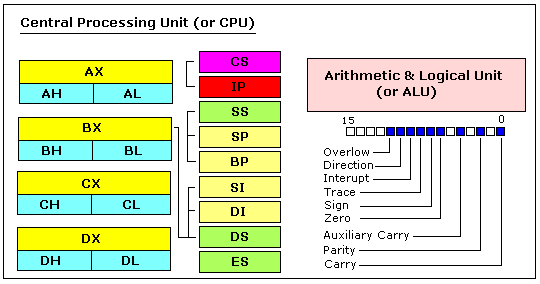
\includegraphics[width=0.8\textwidth]{image/cpu.png}
    \caption{Tổ chức các thanh ghi cơ bản bên trong VXL 8086}
\end{figure}

\subsection{Các thanh ghi đa năng (general purpose registers)}
Vi xử lý 8086 có 8 thanh ghi đa năng gồm:
\begin{itemize}
    \item \code{AX, BX, CX, DX}: các thanh ghi thường sử dụng nhất. Dùng để chứa các tham số đầu vào cũng như kết quả trả về sau khi thực hiện các lệnh.
    \par 4 thanh ghi này có độ dài 16-bit, mỗi thanh ghi được chia làm 2 thanh ghi nhỏ hơn có độ dài 8-bit là \code{AH, AL; BH, BL; CH, CL} và \code{DH, DL}.
    \item \code{SI} (source index): thanh ghi con trỏ nguồn.
    \item \code{DI} (destination index): thanh ghi con trỏ đích.
    \item \code{SP} (stack pointer): thanh ghi trỏ đến đỉnh stack.
    \item \code{BP} (base pointer): ?
\end{itemize}

Tên của các thanh ghi trên được đặt ra bởi những người tạo ra kiến trúc 8086, tuy nhiên những người lập trình có thể sử dụng chúng tuỳ thích phù hợp với mục đích của mình, nhưng phải tuân theo một số quy luật nhất định.\bigskip

Mỗi thanh ghi trong 4 thanh ghi đa năng \code{AX, BX, CX, DX} được chia làm 2 phần gọi là high và low. Ví dụ \code{AX} được cấu thành bởi 2 thành phần là \code{AH} và \code{AL}.\\
Giả sử ta có một số thập phân là \code{12345}. Số này được biểu diễn trong hệ nhị phân là \textcolor{red}{\code{00110000}}\textcolor{blue}{\code{00111001}}\code{b}. Khi ta lưu trữ nó trong thanh ghi \code{AX}, nó sẽ được chia làm 2 phần như sau:

\begin{figure}[H]
    \centering
    \begin{tikzpicture}[mybox/.style={minimum width=3cm,draw,thick,align=center,minimum height=0.5cm}]
        \node[mybox,label=below:\code{AH},text=red] (AH) {\code{00110000}};
        \node[left=1cm of AH] {\code{AX}};
        \node[right=0pt of AH,mybox,label=below:\code{AL},text=blue] (AL) {\code{00111001}};
    
    \end{tikzpicture}
    \caption{Minh hoạ lưu trữ giá trị trong thanh ghi AX.}
\end{figure}

Vì vậy, khi ta thay đổi giá trị của các thanh ghi low và high thì giá trị của thanh ghi lớn cũng bị thay đổi theo và ngược lại.

\subsection{Các thanh ghi đoạn (segment registers)}
\begin{itemize}
    \item \code{CS} (code segment): trỏ đến đoạn bộ nhớ chứa code thực thi của chương trình.
    \item \code{DS} (data segment): trỏ đến đoạn bộ nhớ chứa giá trị của các biến cục bộ.
    \item \code{ES} (extra segment): trỏ đến một đoạn bộ nhớ tuỳ chỉnh. Người sử dụng tự định nghĩa.
    \item \code{SS} (stack segment): trỏ đến đoạn bộ nhớ chứa stack.
\end{itemize}

Để thuận tiện cho việc quản lý, bộ nhớ vật lý trên máy tính được phân chia thành nhiều khu vực logic khác nhau, được gọi là các \textit{đoạn} (segment), mỗi đoạn có mỗi nhiệm vụ khác nhau. Các vùng nhớ cụ thể bên trong các đoạn được gọi là các \textit{offset}.

Ta có thể hiểu đại khái một ``đoạn'' giống như một con đường, còn một offset nằm trong đoạn đó giống như một số nhà nằm trên con đường đó.

Thanh ghi đoạn được sử dụng phối hợp cùng với các thanh ghi đa năng để ghi lại địa chỉ của các ô nhớ. Khi đó thanh ghi đoạn sẽ được sử dụng để chứa địa chỉ đoạn, còn thanh ghi đa năng sẽ được dùng để chứa địa chỉ lệch (offset) của ô nhớ đó tính từ đầu đoạn. Cả 2 kết hợp lại tạo nên \textit{địa chỉ vật lý} của ô nhớ đó.

\begin{figure}[H]
    \centering
    \begin{tikzpicture}
        \node[] (segment) {\bfseries Đường Nguyễn Trung Trực};
        \node[right=1cm of segment] (offset) {\bfseries Số 56};

        \node[below=1cm of segment,align=center] (segment_desc) {Địa chỉ đoạn};
        \node[below=1cm of offset,align=center] (offset_desc) {Địa chỉ lệch\\ \textit{cái nhà thứ 56 tính từ đầu đường}};

        \draw[->, line width=1pt] (segment_desc) edge (segment);
        \draw[->, line width=1pt] (offset_desc) edge (offset);
    \end{tikzpicture}
\end{figure}

Địa chỉ vật lý (physical address) được tạo thành từ địa chỉ trong chỉ 1 thanh ghi đoạn (segment address) và 1 thanh ghi đa năng (offset address) được tính bằng công thức sau:

\begin{center}
\begin{verbatim}
    physical = segment address * 10h + offset.
\end{verbatim}
\end{center}

Vd: Nếu ta có \code{segment address = 1230h} và \code{offset = 45h} (ô nhớ thứ \code{45h} tính từ đầu đoạn \code{1230h}) thì địa chỉ vật lý được tạo từ 2 địa chỉ này là \code{12345h}. Offset còn được gọi là effective address (địa chỉ hiệu quả).\bigskip

Nếu ta có một thanh ghi đoạn là \code{DS} và một thanh ghi đa năng là \code{DX} thì địa chỉ vật lý được tạo bởi 2 địa chỉ chứa trong 2 thanh ghi trên được kí hiệu là \code{DS:DX} và có giá trị là \code{DS * 10h + DX}. 

Vd: Nếu ta có \code{DS = 1230h} và \code{DX = 45h} thì \code{DS:DX = 12345h}.\bigskip

\textbf{Ý nghĩa của thanh ghi đoạn:} giả sử ta có thanh ghi đoạn \code{DS} mang giá trị là \code{1230h} (xem lại định nghĩa của \code{DS} ở trên). Bên trong chương trình, ta khai báo 3 biến sau, mỗi biến chứa 4 byte dữ liệu.
\begin{minted}[]{c}
    a = 123
    b = 456
    c = 789
\end{minted}
Thì biến \code a sẽ có offset là \code 0 (vì nó được khai báo đầu tiên, giống như index \code 0 của phần tử đầu tiên trong mảng). Do \code b nằm ngay sau \code a nên nó sẽ có offset là \code{0 + 4} (do \code a có kích thước là 4 byte). Vậy ta cũng có thể suy ra \code c nằm ở offset số \code 8.

\begin{figure}[H]
    \centering
    \begin{tikzpicture}[mybox/.style={minimum width=3cm,draw,thick,align=center,minimum height=0.5cm}]
        \node[mybox] (a) {\code{123d}};
        \node[right=0pt of a, mybox] (b) {\code{456d}};
        \node[right=0pt of b, mybox] (c) {\code{789d}};

        \node[anchor=east,left=1cm] (DS) at (a.west) {\code{DS=1230h}};
        
        \node[anchor=north] (a_label) at (a.south) {\code{a}};
        \node[anchor=north] (a_offset) at (a_label.south) {\code{Offset 0}};

        \node[anchor=north] (b_label) at (b.south) {\code{b}};
        \node[anchor=north] (b_offset) at (b_label.south) {\code{Offset 4}};

        \node[anchor=north] (c_label) at (c.south) {\code{c}};
        \node[anchor=north] (c_offset) at (c_label.south) {\code{Offset 8}};
    
    \end{tikzpicture}
    \caption{Minh hoạ về offset}
\end{figure}

Như vậy địa chỉ vật lý của 3 biến trên lần lượt là:
\begin{table}[H]
    \centering
    \begin{tabular}{|l|l|l|}
    \hline
    Biến        & Offset    & Physical addr.          \\
    \hline
    \code{a}    & 0         & 1230h * 10h + 0 = 12300h \\
    \code{b}    & 4         & 1230h * 10h + 4 = 12304h \\
    \code{c}    & 8         & 1230h * 10h + 8 = 12308h \\
    \hline
    \end{tabular}
\end{table}

\textbf{Vận dụng:} giả sử \code{a, b, c} mang các kích thước khác nhau lần lượt là \code{2}, \code 4 và \code 6 byte. Hãy cho biết \code{a, b, c} lần lượt thuộc các offset nào và có địa chỉ vật lý là gì? \\
Đáp án:
\begin{table}[H]
    \centering
    \begin{tabular}{|l|l|l|}
    \hline
    Biến        & Offset    & Physical addr.          \\
    \hline
    \code{a}    & 0h         & 1230h * 10h + 0h = 12300h \\
    \code{b}    & 2h         & 1230h * 10h + 2h = 12302h \\
    \code{c}    & 6h         & 1230h * 10h + 6h = 12306h \\
    \code{d}    & 12d = Ch   & 1230h * 10h + Ch = 1230Ch \\
    \hline
    \end{tabular}
\end{table}

\subsection{Các thanh ghi đặc biệt (special purpose registers)}
\begin{itemize}
    \item \code{IP} (instruction pointer): trỏ đến đoạn code đang được thực thi.
    \item Thanh ghi cờ hiệu (flag register): giống như một ``biến toàn cục'' bên trong CPU. Các bit của nó sẽ bị thay đổi giá trị tuỳ thuộc vào kết quả trả về của lệnh mà ta vừa thực hiện trước đó.
\end{itemize}

\subsubsection{Giải thích các bit cờ hiệu phổ biến}
\paragraph{SF (sign flag)}
Sẽ được gán thành \code 1 nếu most significant bit của kết quả của phép tính vừa thực hiện là \code 1, hay nói cách khác, kết quả bị âm. Cờ này mang giá trị \code 0 nếu ngược lại.\break
\textit{Vd:} \code{01001100b + 01100001b =} \textcolor{red}{\code 1}\code{0101101b}.\\ 
Khi đó \code{SF = 1}.
\bigskip

\paragraph{ZF (zero flag)}
Sẽ được gán thành 1 nếu kết quả của phép tính vừa thực hiện là 0.
\bigskip 

\paragraph{PF (parity flag)}
Sẽ được gán thành \code 1 nếu trong kết quả của phép tính vừa rồi có một số \textit{chẵn} các bit \code 1. Nếu không có bit \code 1 nào thì \code{PF} cũng bằng \code 1 (vì 0 cũng là chẵn).\\
\textit{Vd:} \code{01001100b + 01100001b = 10101101b}. Có 5 bit \code 1, nên cờ này sẽ mang giá trị \code 0.

\paragraph{OF (overflow flag)}
\code{OF} được set thành \code 1 nếu như 2 số hạng ban đầu có MSB (bit trái nhất) bằng nhau nhưng tổng của 2 số hạng đó có MSB khác kết quả của 2 số hạng ban đầu.
\begin{itemize}
    \item \codeh{1}\code{111b + }\codeh{1}\code{000b = } \codeh{0}\code{000b} $\Rightarrow$ \code{OF = 1}.
    \item \codeh{0}\code{111b + }\codeh{0}\code{001b = }\codeh{1}\code{111b}. $\Rightarrow$ \code{OF = 1}.
    \item \codeh{1}\code{111b + }\codeh{0}\code{001b = }\codeh{0}\code{000b}. $\Rightarrow$ \code{OF = 0}.
\end{itemize}
Overflow flag chỉ bị tác động bởi phép cộng.

\paragraph{CF (carry flag)}
\code{CF} sẽ mang giá trị \code 1 trong 2 trường hợp dưới đây:
\begin{itemize}
    \item Khi ta thực hiện phép cộng mà số được nhớ nằm ngoài vùng biểu diễn của thanh ghi.
        \begin{verbatim}
            1111b 
          + 0001b 
            -----
           .0000b 
        \end{verbatim}
    Ta thấy khi ta thực hiện xong phép cộng này, vẫn còn 1 số \code 1 được ``nhớ'' ở ngoài cùng bên trái, nhưng nó lại nằm ngoài vùng biểu diễn của thanh ghi này (vì nó chỉ có 4 bit).
    \item Khi ta thực hiện phép trừ mà số được ``mượn'' nằm ngoài vùng biểu diễn của thanh ghi.
        \begin{verbatim}
            0000b 
          - 0001b 
            -----
           .1111b 
        \end{verbatim}
    Ta thấy khi ta thực hiện xong phép trừ này, vẫn còn 1 số \code 1 được ``mượn'' mà chưa trả nằm ở ngoài cùng bên trái của kết quả, nhưng nó lại nằm ngoài vùng biểu diễn của 2 thanh ghi toán hạng, nên ta không thể ``trả'' được.
\end{itemize}

\textit{Lưu ý: CPU không quan tâm phép tính bạn vừa thực hiện là có dấu hay không dấu, 2 số hạng là âm hay dương. Nó chỉ thực hiện việc cộng/trừ trên 2 toán hạng nhị phân và thực hiện việc set cờ tương ứng theo quy luật trên}.\cite{overflow_note}.

\textbf{Một số ví dụ:} 
\begin{figure}[H]
    \centering
    \begin{tabular}{|l|l|l|l|l|l|l|}
    \hline
    Biểu thức                    & SF & ZF & PF & OF & CF \\
    \hline
    \code{1111b + 1000b = 0000b} & 0  & 1  & 1  & 1  & 1 \\
    \code{0101b + 0111b = 1100b} & 1  & 0  & 1  & 1  & 0 \\
    \code{1111b + 0010b = 0001b} & 0  & 0  & 0  & 0  & 1 \\
    \code{1111b - 0011b = 1100b} & 1  & 0  & 1  & 0  & 0 \\
    \code{0000b - 0001b = 1111b} & 1  & 0  & 1  & 0  & 1 \\
    \hline
    \end{tabular}
\end{figure}

%%%%%%%%%%%%%%%%%%%%%%%%%%%%%%%%%%%%%%%%%%%%%%%%%%%%%%%

\section{Cấu trúc chung của một chương trình hợp ngữ 8086}
Có rất nhiều cách để tổ chức một chương trình trong 8086 Asm vì sự đa dạng của compiler hồi đó. Tuy nhiên, ta có cách thường sử dụng sau:

\begin{minted}[linenos]{asm}
.model <kiểu bộ nhớ>
.stack <địa chỉ của SS>

.data
    <khai báo các biến>

.code 
    <khai báo các thủ tục và macro>

    main proc 
        <nội dung hàm main>
    endp

end main ; kết thúc chương trình và nhắc compiler tên của hàm main
\end{minted}
Vd: 
\begin{minted}[linenos]{asm}
.model small
.stack 100h

.data
    strHelloWorld db "Hello world$"

.code 
    printDXString proc 
        mov ah, 09h
        int 21h
    endp

    main proc 
        lea dx, strHelloWorld
        call printDXString
    endp

end main 
\end{minted}

\section{Truy cập bộ nhớ}
\subsection{Sơ lược về truy cập bộ nhớ}
Để truy cập vào một ô nhớ, ta có thể chứa địa chỉ offset của ô nhớ đó trong
\begin{itemize}
    \item Một thanh ghi con trỏ như \code{SI, DI}.
    \item Thanh ghi \code{BX}.
    \item Truy cập trực tiếp vào địa chỉ của ô nhớ đó (displacement). Có 2 loại địa chỉ là địa chỉ 8-bit (\code{d8}) và địa chỉ 16-bit (\code{d16}).
\end{itemize}

\textit{Lưu ý: Địa chỉ được chứa trong các thanh ghi SI, DI, BX hoặc d8, d16 là các địa chỉ offset. Địa chỉ vật lý thực sự của các ô nhớ đó thực chất là \code{DS:SI}, \code{DS:DI}, \code{DS:BX}, \code{DS:d8}, \code{DS:d16}. Cũng cần phải lưu ý một ô nhớ có kích thước là 1 byte}.
\bigskip

Ví dụ: Giả sử hệ điều hành cấp cho ta \code{DS = 1230h}.
Để truy cập vào ô nhớ có địa chỉ vật lý là \code{12345h} bằng thanh ghi \code{SI} thì ta phải gán \code{SI = 45h} vì \code{DS:SI = 1230h * 10h + 45h = 12345h}.

\subsection{Lệnh \code{mov}}
\begin{minted}{asm}
    mov dest, src
\end{minted}
Lệnh \code{mov} nhận vào 2 tham số là \code{src} và \code{dest} và có tác dụng gán giá trị của \code{src} cho \code{dest}.\\
Mã C tương ứng: \code{dest = src;}

2 tham số của lệnh \code{mov} có thể là:
\begin{figure}[H]
    \begin{minipage}{0.5\textwidth}
\begin{verbatim}
SYNTAX 

mov REG, memory
mov memory, REG
mov REG, REG
mov memory, imm
mov REG, imm
mov SREG, memory
mov memory, SREG 
mov SREG, SREG 
mov SREG, REG
\end{verbatim}
    \end{minipage}
    \hfill
        \begin{minipage}{0.5\textwidth}
\begin{verbatim}
VÍ DỤ 

mov AX, [0FFh]
mov [0FFh], AX
mov AX, BX
mov [0CAFEh], 24h
mov AX, 1234h
mov ES, [0445h]
mov [0445h], DS 
mov ES, DS 
mov DS, AX
\end{verbatim}         
         \end{minipage}
\end{figure}

Trong đó:
\begin{itemize}
    \item \code{REG} là một thanh ghi đa năng như \code{AX, BX, SI}.
    \item \code{memory} là một địa chỉ bộ nhớ như \code{[0DEADh], [0BEEFh], [0CAFEh]}.
    \item \code{imm} là một số như \code{1d, 2d, 0FFh, 024h, 1011b}.
    \item \code{SREG} là một thanh ghi đoạn như \code{DS, ES, SS}.
\end{itemize}

Cú pháp \code{[memory]} nghĩa là ``nội dung ô nhớ tại địa chỉ \code{memory}''. Hay nói cách khác, đây là kí hiệu giải tham chiếu tương tự như dấu \code{*} trong C.

\section{Biến và mảng}
\subsection{Giới thiệu về biến}
Biến trong 8086 Asm thường được khai báo ở data segment.
Cú pháp khai báo biến:
\begin{minted}{asm}
<tên biến> <kích thước> <(các) giá trị>
\end{minted}

Tên biến tuân thủ theo các quy tắc đặt tên biến đã biết trước đây.
Kích thước có thể là:
\begin{itemize}
    \item \code{db} (define byte): định nghĩa một biến có kích thước 1 byte.
    \item \code{dw} (define word): định nghĩa biến kích thước 2 byte.
    \item \code{dd} (define double [word]): định nghĩa biến có kích thước 4 byte.
\end{itemize}

Như đã nói ở phần trước, lưu ý rằng khi khai báo, các biến này sẽ nằm trong data segment. Để truy cập vào nội dung các biến này thông qua địa chỉ của chúng, các địa chỉ đó phải là địa chỉ offset được tính từ đầu data segment.

Để có thể truy cập được nội dung của các biến đã khai báo trong data segment, đầu hàm main ta phải có đoạn code sau để nạp địa chỉ của data segment vào thanh ghi \code{DS}:
\begin{minted}[linenos]{asm}
mov ax, @data 
mov ds, ax
\end{minted}

Một số ví dụ về khai báo biến:
\begin{minted}[linenos]{asm}
.data 
    var0 db ?           ; biến 1 byte, giá trị không biết trước
    var1 db 2           ; biến 1 byte, giá trị là 2d
    var2 db 24h         ; biến 1 byte, giá trị là 24h
    var3 db '$'         ; biến 1 byte, giá trị là 24h (mã ASCII của '$')
    var4 dw DEADh       ; biến 2 byte, giá trị là DEADh
    var5 dd DEADBEEFh   ; biến 4 byte, giá trị là DEADBEEFh
\end{minted}

\subsection{Khai báo mảng}
Để khai báo một mảng, ta làm như khai báo biến:
\begin{minted}[linenos]{asm}
.data
    arr1 db 1, 2, 3, 4              ; mảng mà mỗi phần tử là 1 byte
    arr2 dw DEADh, BEEFh, CAFEh     ; mảng có phần tử 2 byte
    arr3 dd DEADBEEFh, 0DEADDADh    ; mảng có phần tử 4 byte
\end{minted}
3 dòng trên tương đương với 3 dòng lệnh C (về mặt \textbf{kích thước} các phần tử):
\begin{minted}[linenos]{c}
char arr1[] = {1, 2, 3, 4};
short arr2[] = {0xDEAD, 0xBEEF, 0xCAFE};
int arr3[] = {0xDEADBEEF, 0xDEADDAD};
\end{minted}

Lưu ý: mảng trong Assembly chỉ là những con trỏ và không thực sự bị giới hạn bởi kích thước khi chúng ta khai báo. Lập trình viên khi code phải tự đảm bảo rằng mình không đi vượt ra khỏi miền giá trị của mảng.

Ngoài ra ta cũng có thể cấp phát (tĩnh) một mảng có kích thước cho sẵn:
\begin{minted}[linenos]{asm}
.data
    arr1 db 100 dup(?)  ; mảng 100 phần tử mà mỗi pt là 1 byte, không có giá trị đầu
    arr2 dw 100 dup(0)
\end{minted}
2 dòng trên tương đương với 2 dòng lệnh C (về mặt \textbf{kích thước} các phần tử):
\begin{minted}[linenos]{c}
char arr1[100];
short arr2[100] = { 0 }; 
\end{minted}

Như trong C, một chuỗi cũng là một mảng, và có kích thước mỗi phần tử là 1 byte (\code{db}).

\subsection{Truy cập vào biến bằng \code{mov}}.
Ta có thể truy cập trực tiếp vào giá trị của biến bằng lệnh mov:
\begin{minted}[]{asm}
var1 db 24h
mov ax, var1    ; ax = 24h
\end{minted}
Ta có thể truy cập gián tiếp thông qua địa chỉ của nó:
\begin{minted}[]{asm}
var1 db 24h            
mov bx, offset var1    ; bx = địa chỉ offset var1
mov ax, [bx]           ; ax = *(ds*10h+bx) 
                       ; Nhắc lại: SI, DI, BX luôn luôn đi ngầm định với DX
\end{minted}

\subsection{Truy cập vào mảng}
Ta có thể truy cập vào mảng bằng cú pháp như trong C (có một số chỗ hơi khác một tí):
\begin{minted}[]{asm}
arr1 db 0Ah, 0Bh, 0Ch, 0Dh, 0Eh 
... 
mov al, arr         ; al = 0Ah 
mov al, arr[0]      ; al = 0Ah 
mov al, arr[2]      ; al = 0Ch 
mov bx, offset arr  ; bx = địa chỉ của arr
mov al, [bx + 3]    ; al = *(bx + 3) = *(arr + 3) = arr[3]
\end{minted}

\subsection{Lệnh \code{lea}}
\code{LEA} là Load Effective Address.\\
Ngoài cách ghi \code{mov REG, offset variable} ta còn có thể ghi là \code{lea REG, variable}.\\
Vd:
\begin{minted}[]{asm}
mov bx, offset var1 
lea bx, var1        ; 2 cách ghi tương đương nhau
\end{minted}

\section{Ngắt (interrupt)}
Các interrupt giống như những ``thư viện chuẩn'' mà hệ điều hành/BIOS cung cấp cho chúng ta. \\
Mỗi interrupt được đánh một số thứ tự nhất định (vd: \code{21h}).\\
Bên trong các interrupt là các hàm hệ thống (syscall).\\
Khi ta muốn gọi một hàm hệ thống nào đó, ta lưu mã số của hàm đó trong thanh ghi \code{AH}, và các thanh ghi còn lại dùng để chứa tham số của hàm đó (thanh ghi nào chứa giá trị gì thì tuỳ vào từng hàm). Cuối cùng ta gọi lệnh \code{int <mã số interrupt>}.\\
Vd:
\begin{minted}[]{asm}
; In một chuỗi được trỏ tới bởi DX ra màn hình 
; Interrupt 21h, hàm số 09h
mov ah, 09h 
lea dx, str 
int 21h
\end{minted} 
Danh sách các interrupt phổ biến: \href{https://jbwyatt.com/253/emu/8086_bios_and_dos_interrupts.html}{\code{8086 BIOS and DOS interrupts}}.

\section{Nhập xuất dữ liệu}
Để nhập xuất dữ liệu trong Assembly, ta không thể làm thủ công mà ta phải nhờ đến các hàm hệ thống có sẵn trong hệ điều hành hoặc BIOS. Dưới đây là một số cú pháp nhập/xuất cơ bản sử dụng API của MS-DOS (\code{int 21h}).

\subsection{Đọc một kí tự từ bàn phím}
\begin{itemize}
    \item Mã hàm: \code{01h}.
    \item Tham số: không.
    \item Trả về: \code{AL = mã ASCII của kí tự vừa đọc}. \code{AL = 0} nếu đó là kí tự điều khiển.
\end{itemize}
\begin{minted}[]{asm}
mov ah, 01h 
int 21h
\end{minted}

\subsection{In một kí tự ra màn hình}
\begin{itemize}
    \item Mã hàm: \code{02h}.
    \item Tham số: \code{DL = mã ASCII của kí tự cần hiển thị}.
    \item Trả về: Không.
\end{itemize}
\begin{minted}[]{asm}
; In kí tự '$' ra màn hình 
mov ah, 02h 
mov dl, '$'     ; hoặc mov dl, 24h (mã ascii của kí tự '$')
int 21h
\end{minted}

\subsection{Hiện chuỗi kí tự ra màn hình}
\begin{itemize}
    \item Mã hàm: \code{09h}.
    \item Tham số: \code{DX = địa chỉ offset của chuỗi}.
    \item Trả về: Không.
    \item Lưu ý: chuỗi cần hiển thị phải kết thúc bằng dấu \code{'\$'}.
\end{itemize}
\begin{minted}[]{asm}
str db "Hello world$"
... 
mov ah, 09h 
mov dx, offset str   ; hoặc lea dx, str
int 21h
\end{minted}
\subsection{Đọc chuỗi kí tự từ bàn phím}
\begin{itemize}
    \item Mã hàm: \code{0Ah}.
    \item Tham số: \code{DX = địa chỉ offset của chuỗi}.
    \item Trả về: \code{[DX+1]}: số ký tự đã đọc. \code{[DX+2]}: chuỗi đã đọc được.
    \item Lưu ý: buffer chuỗi này phải có cấu trúc như sau:
    \begin{verbatim}
<số ký tự tối đa đọc được>, <số ký tự đã đọc>, <phần nội dung đã đọc được>
    \end{verbatim}
    \par Hàm này không tự chèn dấu \code{'\$'} vào cuối chuỗi.
\end{itemize}
\begin{minted}[breaklines]{asm}
str db 100, 0, 100 dup(?)
...
mov ah, 0ah 
mov dx, offset str 
int 21h
\end{minted}
Giải thích:
\begin{itemize}
    \item Cấu trúc của biến \code{str} trong khai báo(từ trái qua phải):
    \begin{itemize}
        \item \code{db}: mỗi phần tử của chuỗi là 1 byte (hiển nhiên).
        \item \code{100}: báo cho hệ điều hành biết được nó có thể đọc tối đa 100 kí tự (giống như số \code 100 trong \code{getline(cin, str, 100)} trong C++).
        \item \code{0}: số kí tự mà hệ điều hành đã đọc được. Hiện tại là \code 0. Sau khi hệ điều hành đọc xong nó sẽ gán giá trị tương ứng cho ô nhớ này.
        \item \code{100 dup(?)}: chuỗi ``thực sự'' mà hệ điều hành sẽ lưu dữ liệu đã đọc được vào đây. Giống như khai báo \code{char str[100]};
    \end{itemize}
    \item Giả sử ta đã nhập vào chuỗi \code{"Dm assembly kho vcl"}. Chuỗi này gồm có 18 ký tự. Biến \code{str} sau khi nhập xong sẽ có giá trị là:
    \begin{verbatim}
100, 18, "Dm assembly kho vcl" <các giá trị rác>
    \end{verbatim} 
    \par Sau chuỗi này là giá trị rác, vì khi khai báo ta đã khai báo một chuỗi có 100 phần tử, nhưng chuỗi đọc được chỉ có 18 phần tử mà thôi. Do đó, 82 phần tử còn lại sẽ là giá trị rác.
\end{itemize}

\section{Các phép toán số học và logic}
\subsection{Phép cộng}
\begin{minted}[]{asm}
add dest, src
\end{minted}
Để thực hiện cộng 2 giá trị, ta sử dụng lệnh \code{ADD}. Lệnh này nhận vào 2 tham số \code{dest} và \code{src} và thực hiện phép gán: \code{dest += src}.\\
\textbf{Chú ý:} 2 toán hạng không được phép là 2 ô nhớ và thanh ghi đoạn.
\begin{minted}[]{asm}
mov ax, 12d 
add ax, 8d  ; ax += 8
            ; ax = 12 + 8 = 20 
\end{minted}
Lệnh này tác động đến các cờ \code{AF, CF, OF, PF, SF, ZF}.

\subsection{Phép trừ}
Lệnh: \code{SUB}. Cú pháp và giới hạn tương tự lệnh \code{ADD}.
\begin{minted}[]{asm}
mov ax, 12d 
mov bx, 2d
sub ax, bx  ; ax -= 2
            ; ax = 12 - 2 = 10 
\end{minted}
Lệnh này tác động đến các cờ \code{AF, CF, OF, PF, SF, ZF}.

\subsection{Phép nhân}
Cú pháp: 
\begin{minted}[]{asm}
mul X
\end{minted}
Lệnh \code{MUL} nhân 2 số không dấu.
Có 2 trường hợp xảy ra:
\begin{itemize}
    \item Nếu \code{X} có kích thước 8 bit (1 byte), lệnh này sẽ thực hiện phép gán: \code{AX = AL * X}.
    \item Nếu \code{X} có kích thước 16 bit (2 byte), lệnh này sẽ thực hiện phép gán: \code{DXAX = AX * X}.
    \par trong đó DXAX là một thanh ghi tổ hợp (tưởng tượng) gồm high là DX và low là AX.
\end{itemize} 
Lệnh này chỉ tác động đến các cờ \code{CF, OF}.


\begin{minted}[breaklines]{asm}
; Demo TH1 
mov al, 5d      ; AL, BL là thanh ghi 8 bit
mov bl, 2d 
mul bl          ; AX = AL * BL = 5 * 2 = 10
; Demo TH2 
mov ax, 5d 
mov bx, 2d 
mul bx          ; DXAX = AX * BX = 5d * 2d = 0010d
                ; Lúc này DX = 0 và AX = 10 vì 10 < FFFFh vẫn đủ nhỏ để nằm trong AX
; Demo TH2 (tt)
mov ax, 0DEADh
mov bx, 0DADh
mul bx          ; DXAX = AX * BX = DEADh * DADh = 0BE543E9h
                ; lúc này DX = 0BE5h và AX = 43E9h vì số trên quá lớn để nằm vừa trong AX
\end{minted}

Ngoài ra ta còn lệnh \code{IMUL} với cú pháp tương tự, nhưng nó sẽ treat 2 toán hạng là 2 số có dấu.

\subsection{Phép chia}
\begin{minted}[]{asm}
div X
\end{minted}
Lệnh \code{DIV} chia 2 số không dấu.
Có 2 trường hợp xảy ra:
\begin{itemize}
    \item Nếu \code{X} có kích thước 8 bit (1 byte), lệnh này sẽ thực hiện phép gán: \code{AL = AX div X} (thương) và \code{AH = AX mod X} (dư).
    \par Biểu diễn dưới dạng chia Euler: \code{AX = X*AL + AH}.
    \item Nếu \code{X} có kích thước 16 bit (2 byte), lệnh này sẽ thực hiện phép gán: \code{AX = DXAX div X} và \code{DX = DXAX mod X}.
    \par Biểu diễn dưới dạng chia Euler: \code{DXAX = X*AX + DX}.
\end{itemize} 
\begin{minted}[]{asm}
; Demo TH1 
mov ax, 120d
mov bl, 10d ; BL là thanh ghi 8 bit 
div bl      ; AL = thương, AH = dư 
            ; AL = 12, AH = 0
; Demo TH1 (tt)
mov ax, 123d 
mov bl, 2d 
div bl      ; AL = thương = 61 
            ; AH = dư = 1
; Demo TH2 
mov dx, 0
mov ax, DEADh   ; ta phải gán DX = 0 để DXAX = AX 
mov bx, BEEFh 
                ; Thực hiện chia DEADh/BEEFh
div bx          ; AX = thương = 1d
                ; DX = dư = 8126d
; Demo TH2 (tt)
mov dx, 0FACh
mov ax, EB00h   ; DXAX = FACEB00h
mov bx, DEADh 
                ; Thực hiện chia FACEB00h/DEADh
div bx          ; AX = thương = 1205h
                ; DX = dư = 679Fh

\end{minted}
Lệnh này không tác động đến cờ.

\subsection{Lệnh \code{INC} và \code{DEC}}
Cú pháp:
\begin{minted}[]{asm}
inc X
dec X
\end{minted}
Tương đương với 2 dòng C sau:
\begin{minted}[]{asm}
X++
X--
\end{minted}
Vd:
\begin{minted}[]{asm}
mov ax, 12d 
inc ax          ; ax = 13d
mov bx, 70d     
dec bx          ; bx = 69d
\end{minted}
2 lệnh này thay đổi cờ tương tự như \code{ADD} và \code{SUB}.

\subsection{Các phép toán logic}
\subsubsection{Lệnh \code{AND}}
\begin{minted}[]{asm}
and dest, src
\end{minted}
Lệnh \code{AND} nhận vào 2 tham số như trên và thực hiện phép gán: \code{dest = dest \& src}.\\
Vd:
\begin{minted}[]{asm}
mov ah, 10110110b
mov al, 01101010b
and ah, al          ; AH = AH and AL 
; KQ: AH = 00100010b
\end{minted}
\begin{verbatim}
    10110110b
  & 01101010b
    ---------
    00100010b
\end{verbatim}

\subsubsection{Lệnh \code{OR}, \code{XOR}}
Tương tự lệnh \code{AND}.
\begin{minted}[]{asm}
mov ah, 10110110b
mov al, 01101010b
or ah, al          ; AH = AH or AL 
; KQ: AH = 11111110b
\end{minted}

\subsubsection{Lệnh \code{NOT}}
\begin{minted}[]{asm}
not X
\end{minted}
Lệnh \code{NOT} nhận vào 1 tham số như trên và thực hiện phép gán: \code{X = not X} (đảo các bit của \code X).
Vd:
\begin{minted}[]{asm}
mov ah, 10110110b
not ah
; KQ:   01001001b
\end{minted}

\subsubsection{Lệnh \code{NEG}}
Cú pháp:
\begin{minted}[]{asm}
neg X
\end{minted}
Lệnh này thực hiện đảo dấu của X bằng cách thực hiện lấy số bù 2.
Vd:
\begin{minted}[]{asm}
mov ax, 01101100b
neg ax 
; ax = 10010100b
\end{minted}

\subsubsection{Các lệnh dịch bit}
Có 2 lệnh dịch bit là \code{SHL} (shift left) và \code{SHR} (shift right). Chúng hoạt động giống toán tử \verb#<<# và \verb#>># trong C và có syntax tương tự nhau:
\begin{minted}[]{asm}
shl X
shr X
\end{minted}
2 lệnh trên để dịch \code X qua trái (phải) 1 bit. Kết quả dịch sẽ được gán lại trực tiếp vào thanh ghi \code X, và bit bị ``rơi ra'' sẽ nằm trong thanh ghi cờ \code{CF}.\\
Vd:
\begin{minted}[]{asm}
mov ah, 10010001b
shl ah 
; AH << 1 => AH = 00100010b, CF = 1

mov ah, 10011100b
shr ah 
; AH >> 1 => AH = 01001110b, CF = 0
\end{minted}
Ngoài ra ta còn có thể dịch nhiều bit cùng lúc:
\begin{minted}[]{asm}
shl X, Y 
shr X, Y
\end{minted}
Mã C tương ứng:
\begin{minted}[]{asm}
X << Y 
X >> Y
\end{minted}

\section{Các cấu trúc điều khiển}

\section{Cách chuyển cấu trúc điều khiển C sang Assembly}

\section{Thủ tục}

\section{Macro}

\section{Stack}

\chapter{Một số chương trình cơ bản bằng Assembly 8086} \label{chapterBaiTap}



\renewcommand{\bibname}{Tài liệu tham khảo}
\bibliographystyle{IEEEtran}
\bibliography{references}
\end{document}

%%%%%%%%%%%%%%%%%%%%%%%%%%%%%%%%%%%%%%%%%%%%%%%%%%%%
% Comments can be added to the margins of the document using the \todo{Here's a comment in the margin!} todo command, as shown in the example on the right. You can also add inline comments too:

% \todo[inline, color=green!40]{This is an inline comment.}



% \subsection{Tables and Figures}

% Use the table and tabular commands for basic tables --- see Table~\ref{tab:widgets}, for example. You can upload a figure (JPEG, PNG or PDF) using the files menu. To include it in your document, use the includegraphics command as in the code for Figure~\ref{fig:frog} below.

% % % Commands to include a figure:
% % \begin{figure}
% % \centering
% % \includegraphics[width=0.5\textwidth]{frog.jpg}
% % \caption{\label{fig:frog}This is a figure caption.}
% % \end{figure}

% % \begin{table}
% % \centering
% % \begin{tabular}{l|r}
% % Item & Quantity \\\hline
% % Widgets & 42 \\
% % Gadgets & 13
% % \end{tabular}
% % \caption{\label{tab:widgets}An example table.}
% % \end{table}

% \subsection{Mathematics}

% \LaTeX{} is great at typesetting mathematics. Let $X_1, X_2, \ldots, X_n$ be a sequence of independent and identically distributed random variables with $\text{E}[X_i] = \mu$ and $\text{Var}[X_i] = \sigma^2 < \infty$, and let
% $$S_n = \frac{X_1 + X_2 + \cdots + X_n}{n}
%       = \frac{1}{n}\sum_{i}^{n} X_i$$
% denote their mean. Then as $n$ approaches infinity, the random variables $\sqrt{n}(S_n - \mu)$ converge in distribution to a normal $\mathcal{N}(0, \sigma^2)$.

% \subsection{Lists}

% You can make lists with automatic numbering \dots

% \begin{enumerate}
% \item Like this,
% \item and like this.
% \end{enumerate}
% \dots or bullet points \dots
% \begin{itemize}
% \item Like this,
% \item and like this.
% \end{itemize}

% We hope you find write\LaTeX\ useful, and please let us know if you have any feedback using the help menu above.

